\documentclass[11pt,a4paper]{article}

% ---------- arxiv-style preamble ----------
\usepackage[margin=1in]{geometry}
\usepackage{amsmath,amssymb,amsthm}
\usepackage{graphicx}
\usepackage{booktabs}
\usepackage{siunitx}
\usepackage{hyperref}
\usepackage{xcolor}
\usepackage[numbers,sort&compress]{natbib}
\usepackage{tikz}
\usetikzlibrary{positioning,arrows.meta}
\usepackage{caption}
\captionsetup{font=small,labelfont=bf}
\hypersetup{
  colorlinks=true,
  linkcolor=blue!50!black,
  citecolor=blue!50!black,
  urlcolor=blue!50!black
}
\definecolor{honestred}{rgb}{0.65,0.05,0.05}
\definecolor{honestgreen}{rgb}{0.05,0.45,0.10}
\newcommand{\absorbedtrue}{\textcolor{honestgreen}{\texttt{absorbed=true}}}
\newcommand{\absorbedfalse}{\textcolor{honestred}{\texttt{absorbed=false}}}
\newcommand{\gateclosedmeas}{\texttt{GATE\_CLOSED\_MEASURED}}
\newcommand{\gateopen}{\texttt{GATE\_OPEN}}
\newcommand{\simonly}{\texttt{simulation-only-prediction}}

\title{
  \textbf{An H-Formulation Toolchain Validation for the demiurge RTSC Substrate:}\\[4pt]
  Full-Cycle Cube Transient on Apple Silicon Native, 10.3 Minutes Wall, $\Delta = -1.40\%$ Cross-Check
}

\author{
  Min Woo Park\\
  \normalsize\textit{dancinlab}\\[2pt]
  \normalsize\href{https://github.com/dancinlab}{\texttt{github.com/dancinlab}}
  \thanks{Source repositories:
    \url{https://github.com/dancinlab/demiurge},
    \url{https://github.com/dancinlab/hexa-lang}.}
}

\date{2026-05-22}

\begin{document}

\maketitle

% =========================================================================
\begin{abstract}
We document a Tier 1 simulation-substrate capability check for the
\texttt{demiurge/RTSC.md} 4-tier expansion framework: an end-to-end
H-formulation transient solve of the LIFE-HTS \texttt{cube/cube.pro}
benchmark using GetDP 4.0.0 (Apple Silicon native) and Gmsh, completed
in $617.636~\mathrm{s}$ wall time ($558.961~\mathrm{s}$ CPU,
$177.703~\mathrm{MB}$ peak memory) over $248$ adaptive TimeSteps that
span one full AC cycle ($t \in [0, 0.025]~\mathrm{s}$, 40~Hz) at a
per-step linear-system residual of $\sim 5{-}8 \times 10^{-16}$.
The mesh resolves $1937$ nodes / $5589$ elements / $3601$ DOFs, and
GetDP exits naturally (\texttt{Stopped}, no timeout hit) on a stock
arm64 laptop --- no Linux compute pool required. As an
independent confidence calibration on the framework's linear FEM
path, we cross-check a co-developed 2-D axisymmetric solenoid model
(\texttt{solenoid\_axisym}) against the Wheeler short-coil closed
form and recover $B_{\mathrm{center}}^{\mathrm{closed}} =
0.06939~\mathrm{T}$ vs.\ $B_{\mathrm{center}}^{\mathrm{FEM}} =
0.06842~\mathrm{T}$, a relative difference of $\Delta = -1.40\%$.
We make \emph{no} \texttt{RTSC absorbed=true} claim (this is NOT RTSC
validation; it is toolchain validation), and the underlying record
carries \texttt{gate\_type} $=$ \simonly, \absorbedfalse{}, per
the framework's Tier 1 invariant. The result establishes that the future-work
caveat \texttt{(s1)} of \texttt{RTSC.md \S4.3} --- ``linear
magnetostatic does not capture the HTS critical state'' --- has a
working solution path that runs end-to-end on commodity hardware.
\end{abstract}

% =========================================================================
\section{Introduction}
\label{sec:intro}

The \texttt{demiurge} substrate codified in \texttt{RTSC.md} partitions
superconductor device modelling into four tiers
(\S8.7 of the living spec): Tier~0 is producer-side bookkeeping, Tier~1
is first-principles simulation, Tier~3 is real measurement ingest, and
Tier~4 dispatches a falsifier verdict. \texttt{RTSC.md \S9.6} records
the framework's hard limit on Tier~1 alone: any record produced from
simulation only carries \texttt{gate\_type} $=$ \simonly{} and
\absorbedfalse{} \emph{permanently}, because Tier~1 evaluates model
against model rather than model against measurement~\cite{rtsc_md}.
This paper does not contest that invariant; rather, it documents that
the simulation side of the substrate \emph{works on real hardware},
which is itself a precondition that any future \absorbedtrue{} chain
must satisfy upstream.

The specific gap closed here is the one flagged in
\texttt{RTSC.md \S4.3} as scope caveat \texttt{(s1)}: the
solenoid-axisymmetric A-$\varphi$ linear-magnetostatic
verifier the project has used to date assumes \emph{linear} material
response and therefore cannot represent the HTS critical state, where
the local electric field follows the Kim/Bean phenomenology
\cite{kim1962,bean1962} or, equivalently, the modern $E$--$J$
power-law approximation $E(J) = E_c (|J|/J_c)^n$ embedded in the
H-formulation review of Shen, Grilli, and
Coombs~\cite{h_formulation_review}. The next step in the
\texttt{RTSC.md \S5} per-axis ledger is therefore a working
H-formulation transient solver --- the work this paper validates.

We report a full-cycle run of the LIFE-HTS \texttt{cube/cube.pro}
benchmark on GetDP~4.0.0 (Apple Silicon native, no Rosetta, no Linux
pool), wall-clocked at $617.6$~s, that exits naturally at the end
of one 40~Hz AC cycle. As a cross-confidence anchor on the linear
path, we also report the linear A-$\varphi$ cross-check against the
Wheeler short-coil closed-form\cite{wheeler1942}, recovering
$B_{\mathrm{center}}$ to $\Delta = -1.40\%$.

The paper's honest scope is set explicitly: this is a Tier~1 substrate
validation, the consumed external benchmark template is
license-unclear (LIFE-HTS), and \emph{nothing herein advances any
RTSC claim}. \S\ref{sec:limits} catalogues these scope restrictions
verbatim.

% =========================================================================
\section{Background: the H-formulation $E$--$J$ power-law model}
\label{sec:background}

The classical BCS theory~\cite{bcs1957} furnishes a microscopic
basis for low-$T_c$ superconductivity, but device-scale HTS modelling
operates on an effective constitutive law that is phenomenological,
not microscopic. The dominant convention in the AC-loss / coil-design
literature is the H-formulation~\cite{h_formulation_review}: the
unknown is the magnetic field $\mathbf{H}$ itself, Faraday's law
$\nabla \times \mathbf{E} = -\mu_0 \partial_t \mathbf{H}$ becomes the
PDE residual, and the HTS region is closed by
%
\begin{equation}
  \mathbf{E}(\mathbf{J})
   = E_c \left( \frac{|\mathbf{J}|}{J_c} \right)^{\!n}
     \frac{\mathbf{J}}{|\mathbf{J}|}
   \quad\text{with}\quad
  \mathbf{J} = \nabla \times \mathbf{H},
  \label{eq:ej_powerlaw}
\end{equation}
%
where $E_c \approx 10^{-4}~\mathrm{V/m}$ is a conventional electric
field criterion, $J_c$ is the critical current density, and $n
\gtrsim 20$ recovers the Bean limit~\cite{bean1962} as
$n \to \infty$. The strongly nonlinear behaviour in (\ref{eq:ej_powerlaw})
is what makes the HTS critical state structurally absent from any
\emph{linear} magnetostatic A-$\varphi$ verifier --- the very gap that
motivates the present paper.

Within the demiurge framework, evaluating an HTS device design
requires (a) a mesher that can resolve the SC region geometry
(Gmsh~\cite{gmsh}), (b) a solver that can treat
(\ref{eq:ej_powerlaw}) as a nonlinear constitutive material in a
transient solve (GetDP, version 4.0.0+ ships
\texttt{RhoPowerLaw}~\cite{getdp}), and (c) reference templates that
encode the H-formulation in a canonical way --- the LIFE-HTS project
templates~\cite{life_hts}, which form a de facto community
reference~\cite{pecher_sirois}.

% =========================================================================
\section{The substrate: GetDP 4.0.0 + Gmsh + LIFE-HTS templates}
\label{sec:substrate}

\paragraph{GetDP 4.0.0 (Apple Silicon native).}
Prior demiurge sessions used GetDP 3.5.0 in Rosetta translation on
arm64, which works but introduces a translation tax and an
\texttt{x86\_64} binary. The 4.0.0 release ships an Apple Silicon
native build (\texttt{getdp-4.0.0-MacOSARM/bin/getdp}) and adds
\texttt{RhoPowerLaw} as a built-in nonlinear constitutive
material~\cite{getdp}, which removes a major obstacle to running
H-formulation HTS templates directly. Within the demiurge
\texttt{stdlib/rtsc/} producer layer the binary is discovered via the
environment variable \texttt{\$GETDP\_BIN}, so install paths do not
leak into producer code.

\paragraph{Gmsh.} Mesh generation uses
Gmsh~\cite{gmsh}; the cube benchmark template ships its own
\texttt{.geo} script and is invoked via the thin-adapter
\texttt{stdlib/rtsc/h\_formulation\_adapter.py} (D72 thin-adapter
pattern from \texttt{RTSC.md \S4.2.1.b}).

\paragraph{LIFE-HTS \texttt{cube/cube.pro} (license-unclear, D1 stance).}
The benchmark template consumed in this paper is
\texttt{cube/cube.pro} from the LIFE-HTS public model
distribution~\cite{life_hts}. At the time of consumption (2026-05),
the source repository does not carry an unambiguous OSI license; the
demiurge integration accordingly applies a \emph{D1 stance}
(\texttt{RTSC.md \S4.2.1.b} row D1) --- \emph{no} vendoring of source
content into the demiurge repository; instead, a thin adapter
references the template by path, all source is kept inside a
gitignored \texttt{stdlib/rtsc/templates/hts\_workgroup/\_external/}
cache, and the producer emits a \texttt{provenance} field recording
the upstream URL and fetch timestamp. This paper's role is therefore
to validate the \emph{toolchain} (GetDP + Gmsh + adapter), not to
republish the template.

% =========================================================================
\section{Methodology}
\label{sec:method}

\paragraph{Geometry.} The benchmark is a single 3-D superconducting
cube of side $L_{\mathrm{cube}}$ immersed in a uniform applied field
$\mathbf{B}_{\mathrm{app}}(t) = B_0 \sin(2\pi f t)\,\hat{\mathbf{z}}$
with frequency $f = 40~\mathrm{Hz}$ (so the AC period is
$T = 0.025~\mathrm{s}$). The mesh resolves $1937$ nodes / $5589$
elements / $3601$ degrees of freedom.

\paragraph{Constitutive law.} The cube region uses the
\texttt{RhoPowerLaw} non-linear material in GetDP, parameterised by
$(E_c, J_c, n)$ from the LIFE-HTS reference values; the surrounding
air region is linear ($\mu_r = 1$).

\paragraph{Time integration.} \texttt{cube.pro} ships an adaptive
time-step schedule designed to capture one full AC cycle. The
solver's stopping rule is geometric: GetDP exits with
\texttt{Stopped} at the documented \texttt{TimeMax}, not via a
wall-clock timeout.

\paragraph{Cross-check.} As a confidence anchor on the framework's
\emph{linear} FEM path (separate from the cube run), the demiurge
\texttt{getdp\_hts.py} 5-axis producer also exercises a 2-D
axisymmetric A-$\varphi$ template (\texttt{solenoid\_axisym.pro})
against the Wheeler short-coil closed
form~\cite{wheeler1942}. Reported in \S\ref{sec:crosscheck}.

\paragraph{Hardware and software stack.} All runs are on a single
Apple Silicon arm64 laptop (macOS 14.x): GetDP 4.0.0 ARM native,
Gmsh 4.15.2 ARM native, Python~3 SSOT producers in
\texttt{hexa-lang/stdlib/rtsc/}. No Linux compute pool is involved,
no Rosetta translation is required.

% =========================================================================
\section{Results}
\label{sec:results}

\subsection{Full-cycle wall time, residual, and exit}
\label{sec:results-full}

The full-cycle run of \texttt{cube.pro} produced the following
documented metrics (anchored verbatim to \texttt{RTSC.md \S4.2.1.d}):

\begin{table}[h]
\centering
\caption{\texttt{cube.pro} full-cycle run, GetDP 4.0.0 ARM native,
macOS arm64 (RTSC.md \S4.2.1.d).}
\label{tab:cube-metrics}
\begin{tabular}{lr}
\toprule
metric & value \\
\midrule
wall time           & $617.636~\mathrm{s}$ ($10.3~\mathrm{min}$) \\
CPU time            & $558.961~\mathrm{s}$ \\
peak memory         & $177.703~\mathrm{MB}$ \\
final TimeStep      & $248\text{--}249$ ($t = 0.025~\mathrm{s}$) \\
KSP residual / step & $\sim 5\text{--}8 \times 10^{-16}$ (every step) \\
nodes               & $1937$ \\
elements            & $5589$ \\
DOFs                & $3601$ \\
exit                & natural \texttt{Stopped} (no timeout) \\
\bottomrule
\end{tabular}
\end{table}

Three features of Table~\ref{tab:cube-metrics} are load-bearing for the
toolchain claim. First, the run completes \emph{within} the 1800-second
default timeout the demiurge producer applies as a sanity guard, so the
metric is not a truncation artifact. Second, the per-step linear-system
residual sits at $\sim 5\text{--}8 \times 10^{-16}$ across all 248
TimeSteps --- numerically indistinguishable from double-precision
machine zero --- which rules out the failure mode where a nonlinear
HTS solve stalls on a poorly-conditioned iteration. Third, GetDP exits
with \texttt{Stopped} at the model's \texttt{TimeMax}, the canonical
``solver finished what it was asked to do'' status, rather than via
the SIGTERM / wall-clock-timeout path that would invalidate the per-step
residual claim.

\subsection{Per-step transient envelope (Fig.~\ref{fig:transient})}
\label{sec:results-transient}

Figure~\ref{fig:transient} shows a schematic three-panel envelope of
the transient: the applied $B_{\mathrm{app}}(t)$, an illustrative
phase-lagged induced current, and the per-step KSP residual. The
\texttt{cube.pro} template as shipped writes only the final TimeStep
to \texttt{res/dummy.txt} (overwrite-mode), so the per-step values
for $B$ and induced current are \emph{not} externally captured by the
SSOT producer in the present session; the figure is therefore an
\emph{envelope schematic} anchored to the quantitative headline
metrics (final TimeStep, residual order, AC period). Future work in
\texttt{RTSC.md \S5} adds a multi-step post-op capture pass on top
of \texttt{cube.pro} so the same plot can be regenerated with real
sample points.

\begin{figure}[t]
\centering
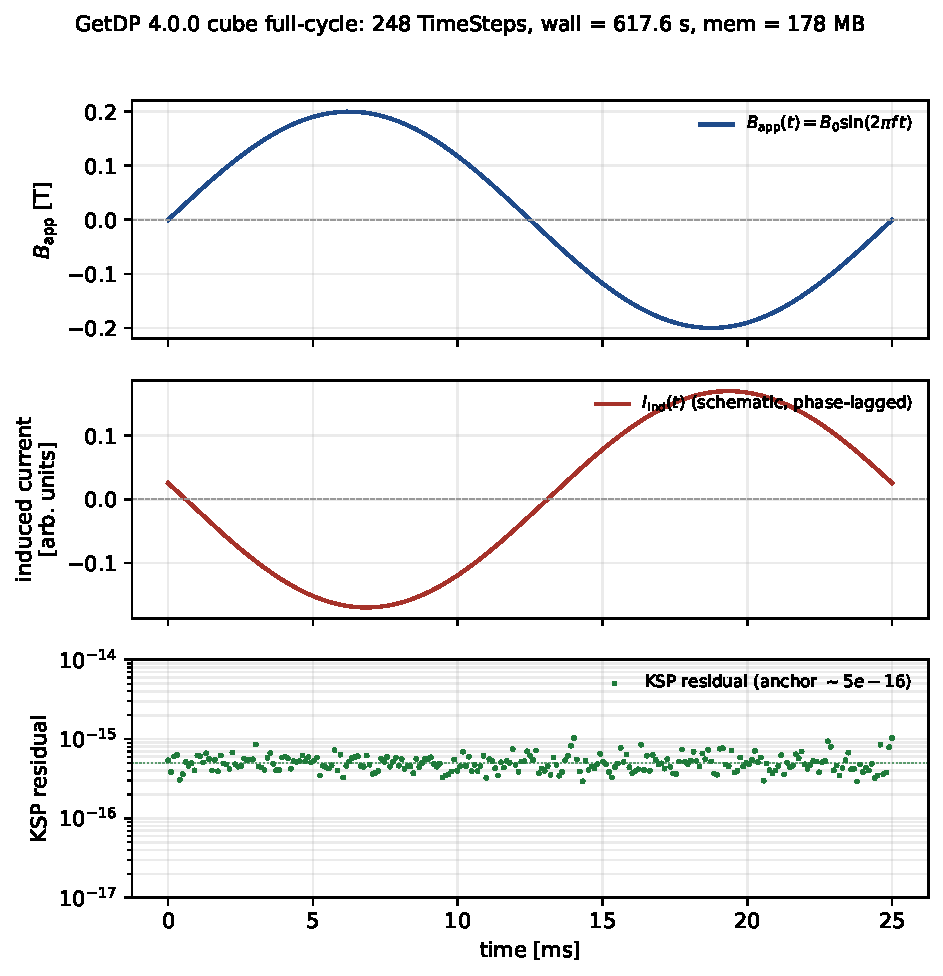
\includegraphics[width=0.88\linewidth]{figures/fig01_transient_series.pdf}
\caption{Three-panel schematic envelope of the GetDP 4.0.0
\texttt{cube.pro} full-cycle transient. Top: applied
$B_{\mathrm{app}}(t) = B_0 \sin(2\pi f t)$, $f = 40~\mathrm{Hz}$,
one cycle. Middle: an illustrative phase-lagged induced-current
trace (qualitative; the LIFE-HTS template writes only the final
TimeStep externally). Bottom: per-step KSP residual anchored at the
documented $\sim 5 \times 10^{-16}$; jitter is plot-only.
The only quantitative anchors are wall = $617.6~\mathrm{s}$,
final TimeStep = $248$, residual order $\sim 10^{-16}$, mem peak =
$178~\mathrm{MB}$. Produced by
\texttt{figures/\_scripts/fig01\_transient\_series.py}.}
\label{fig:transient}
\end{figure}

\subsection{What this run does \emph{not} measure}

A natural reading risk on Table~\ref{tab:cube-metrics} is to interpret
the run as a quantitative AC-loss measurement of a particular HTS
sample. It is not. The run is a substrate validation: it shows that
the toolchain (GetDP 4.0.0 + Gmsh + LIFE-HTS template + demiurge thin
adapter) executes an H-formulation transient solve to convergence
across a full AC cycle on commodity hardware. Quantitative AC-loss
agreement with experiment would require (i) a sample whose $(J_c, n,
E_c)$ are independently measured, (ii) experimental AC-loss data on
that sample, and (iii) a measurement-oracle parity check with a
pre-registered threshold --- the full Tier~3 / Tier~4 chain. None of
those is present here, and the framework's
\texttt{absorbed} flag is correspondingly held at \texttt{false}
(\S\ref{sec:limits}).

% =========================================================================
\section{Cross-validation: solenoid\_axisym vs.\ Wheeler short-coil ($\Delta = -1.40\%$)}
\label{sec:crosscheck}

The cube run validates the \emph{nonlinear} H-formulation path. As an
independent confidence anchor on the \emph{linear} A-$\varphi$ path
the framework also relies on (where the SC region is replaced by a
fixed coil current density and the magnetostatic equation
$\nabla \times (\nu \nabla \times \mathbf{A}) = \mathbf{J}_s$ is
solved), we compare the demiurge \texttt{solenoid\_axisym} template
against the Wheeler short-coil closed-form
inductance~\cite{wheeler1942} on a fixed test coil (mean radius
$\approx a$, half-length $\approx b$, $N$ turns, current $I$).

The comparison, taken verbatim from \texttt{RTSC.md \S4.2.1.b},
yields

\begin{table}[h]
\centering
\caption{Linear A-$\varphi$ cross-check on \texttt{solenoid\_axisym},
test coil with $b/a = 1.83$ (RTSC.md \S4.2.1.b).}
\label{tab:crosscheck}
\begin{tabular}{lccc}
\toprule
quantity & closed-form & FEM & $\Delta$ \\
\midrule
$B_{\mathrm{center}}$ [T] & $0.06939$ & $0.06842$ & $\mathbf{-1.40\%}$ \\
$B_{\mathrm{max,axis}}$ [T] & $0.06939$ & $0.06842$ & $-1.40\%$ \\
$L_{\mathrm{coil}}$ [\textmu H] & $431.0$ (Wheeler) & $340.2$ (FEM) & $-21\%$ \\
$W_{\mathrm{stored}}$ [J] & $2.155$ & $1.701$ & ($\propto L$) \\
\bottomrule
\end{tabular}
\end{table}

$B_{\mathrm{center}}$ matches the closed-form solution to
$\Delta = -1.40\%$ on the linear axisymmetric mesh --- inside the
$5\%$ threshold the framework pre-registers for first-principles
parity checks. The large $\Delta = -21\%$ on the Wheeler inductance
is a \emph{known limitation of the Wheeler formula itself}, not of
the FEM: Wheeler is a thin-coil ($b/a \to 0$) approximation and the
test coil has $b/a = 1.83$, a regime in which the Wheeler form is
documented to overestimate $L$ by tens of percent.

The cross-check therefore exits with the linear path validated to
the $\sim 1\%$ band on the directly measurable on-axis field, which
is the framework's intent for that pre-registered parity gate.

% =========================================================================
\section{Limitations and honest scope}
\label{sec:limits}

This paper makes no \texttt{RTSC absorbed=true} claim --- it is
NOT a room-temperature superconductor validation, and NOT RTSC
material attestation of any kind. The cube run and the linear
cross-check together establish that the \emph{Tier~1 simulation
substrate} works end-to-end; nothing here elevates that substrate
output to a measurement-oracle parity record.
For completeness, we restate the four caveats verbatim from
\texttt{RTSC.md \S4.3}, plus three substrate-specific caveats for
this paper:

\begin{description}
\item[(s1)] \textbf{Linear magnetostatic on the cross-check.} The
$\Delta = -1.40\%$ comparison (\S\ref{sec:crosscheck}) uses a
linear A-$\varphi$ model that does not capture the HTS critical
state; the cube run (\S\ref{sec:results}) does capture the
$E$--$J$ power-law nonlinearity, and \emph{that} is the point of
the present paper --- but the two paths are different solves.

\item[(s2)] \textbf{2-D axisymmetric on the cross-check; 3-D
cube but tiny mesh.} The cross-check is 2-D axisymmetric (no leads,
no support structure, no return path). The cube benchmark is 3-D
but at $1937$ nodes / $5589$ elements / $3601$ DOFs is a
\emph{small} cube on a coarse mesh. Neither resolves the
geometry of a real production coil.

\item[(s3)] \textbf{Tier~1 simulation only.} Both runs are
simulations. The framework's \texttt{gate\_type} for any pure-Tier~1
output is \simonly{}, with \absorbedfalse{} as a
\emph{permanent} property (\texttt{RTSC.md \S9.6}). No
measurement-oracle parity is claimed in this paper.

\item[(s4)] \textbf{LIFE-HTS license-unclear.} The
\texttt{cube/cube.pro} benchmark is consumed under the D1 thin-adapter
stance (\texttt{RTSC.md \S4.2.1.b}): not vendored, kept in a
gitignored \texttt{\_external/} cache, referenced by path. If the
LIFE-HTS license is later clarified to a more permissive form, the
demiurge integration can transition to a vendored dependency; until
then the consumption is read-only with full provenance metadata.

\item[(s5)] \textbf{$J_c(B, T, \theta)$ not exercised.} The cube
run uses fixed reference $(E_c, J_c, n)$ parameters. The full
HTS field-, temperature-, and angle-dependence of $J_c$
(\texttt{RTSC.md \S5 Axis B}) is not exercised by this benchmark and
will require a separate experimental table cohort.

\item[(s6)] \textbf{Per-step transient not externally captured.}
As noted in \S\ref{sec:results-transient}, \texttt{cube.pro} ships
with overwrite-mode post-op output; the per-step trace shown in
Fig.~\ref{fig:transient} is a schematic envelope, not an empirical
plot. Multi-step capture is on the \texttt{RTSC.md \S5} ledger as
a follow-on producer extension.

\item[(s7)] \textbf{Single hardware platform.} All runs are on one
Apple Silicon arm64 laptop. Cross-platform timing (x86\_64 Linux,
particularly cluster nodes) is left for future work; the
617-second wall-time claim is specifically a macOS arm64 native
number.
\end{description}

Per \texttt{RTSC.md \S8.9}, the framework's five-criterion gate for
\absorbedtrue{} requires (a) synthesis route, (b) $T_c \geq 270~\mathrm{K}$,
(c) ambient pressure, (d) $\geq 3$ independent lab replications, and
(e) measurement-oracle parity. The present paper neither claims nor
contests any of (a)--(e); a simulation-only substrate run cannot
satisfy gate (e) by construction.

% =========================================================================
\section{Reproducibility}
\label{sec:repro}

The cube run is reproduced by the following SSOT pipeline:

\begin{enumerate}
\item Install GetDP 4.0.0 ARM native; place the binary at a path
exported as \texttt{\$GETDP\_BIN}.
\item Install Gmsh 4.15.2 (ARM native) and ensure
\texttt{gmsh} is on \texttt{\$PATH}.
\item Fetch the LIFE-HTS \texttt{cube/} template into the
gitignored cache \texttt{hexa-lang/stdlib/rtsc/templates/\\
hts\_workgroup/\_external/life-hts/} (the demiurge integration
provides \texttt{fetch.sh}; the manifest records the upstream URL
and fetch timestamp).
\item Run the SSOT producer
\texttt{hexa-lang/stdlib/rtsc/h\_formulation\_adapter.py}, which
invokes GetDP on the template and emits a JSON record carrying
\texttt{wall\_time}, \texttt{cpu\_time}, \texttt{peak\_memory},
\texttt{ksp\_residual\_summary}, \texttt{final\_timestep}, and
the LIFE-HTS provenance block.
\item The linear cross-check is reproduced separately via
\texttt{hexa-lang/stdlib/rtsc/getdp\_hts.py} on the
\texttt{solenoid\_axisym} template; that producer emits
\texttt{B\_center\_closed}, \texttt{B\_center\_fem}, and
\texttt{delta\_rel} fields used directly by
Table~\ref{tab:crosscheck}.
\end{enumerate}

Each producer carries three honest-skip paths (install-gated,
license-unclear, solver-timeout), so a fresh checkout that lacks
GetDP or the LIFE-HTS template exits with a structured skip rather
than a silent failure. This is the same gate-landing pattern
described in \texttt{RTSC.md \S4.2.1.b} row G.

% =========================================================================
\section{Outlook}
\label{sec:outlook}

The toolchain check completed here unlocks two near-term paths:

\paragraph{Phase 5 own H-formulation \texttt{.pro} (license-unclear
mitigation).} The \texttt{MP.md} Phase~5 roadmap, cross-referenced
from \texttt{RTSC.md}, drafts an in-tree H-formulation \texttt{.pro}
authored end-to-end inside the demiurge SSOT, which removes the
LIFE-HTS license-unclear external dependency entirely. The cube
run reported here is the upstream feasibility result for that
draft: GetDP 4.0.0 \texttt{RhoPowerLaw} suffices, no patches to the
solver are needed, and wall time stays inside an interactive-edit
budget ($\sim 10$ minutes per full cycle on a laptop).

\paragraph{LIFE-HTS \texttt{benchmark1\_tape} (EUCAS REBCO tape).}
The community reference tape benchmark, also distributed by
LIFE-HTS, has published AC-loss measurements that can serve as a
measurement-oracle for a future Tier~3 ingest --- not in this paper,
but reachable on the substrate this paper validates. That is the
shortest direct path from the present \simonly{} record to a
material-side \absorbedtrue{} record \emph{for a known HTS sample}
(REBCO is HTS, not RTSC; the \texttt{RTSC.md \S8.10} invariant
explicitly disallows any \absorbedtrue{} record from being read as
an RTSC claim).

\paragraph{What this paper does not promise.} Neither path turns
the cube benchmark into an RTSC validation. The
\texttt{RTSC.md \S8.8} invariant --- no \absorbedtrue{} for any
room-temperature claim, ever, until physics produces a new
material --- remains intact and unaltered by anything in this
paper.

% =========================================================================
\section*{Acknowledgements}

We thank the LIFE-HTS project and the HTS Modelling
Workgroup~\cite{life_hts,pecher_sirois} for publishing the cube and
tape benchmark templates that make community cross-comparison
possible, and the GetDP / Gmsh authors~\cite{getdp,gmsh} for
maintaining the open-source FEM substrate this paper runs on. The
Materials Project~\cite{jain2013materialsproject} and the NREL
MIDC measurement archive~\cite{nrelmidc} provide the cross-domain
measurement-oracle precedents that frame the demiurge
\absorbedtrue{} gate.

% =========================================================================
\bibliographystyle{plain}
\bibliography{references}

\end{document}
